\documentclass[11pt]{article}
\usepackage[margin=0.82in]{geometry}
\usepackage{amsmath,amssymb,booktabs,graphicx,hyperref,placeins,microtype,xcolor}
\hypersetup{colorlinks=true,linkcolor=blue!45!black,urlcolor=blue!45!black}
\setlength{\parindent}{0pt}\setlength{\parskip}{5pt}
\newcommand{\scri}{\mathscr I^+}
\newcommand{\dt}{\mathcal D_t}
\newcommand{\A}{\mathcal A}
\title{A local hyperbolic shift with exact scri nullness\\\large Spherical prototype, boundary closure, and qualification failures}
\author{Numerical formulation note}
\date{27 October 2026}
\begin{document}
\maketitle
\begin{abstract}
We replace the elliptic shift by an auxiliary Gamma driver while retaining the full variable-metric spherical Z4c equations. Algebraic elimination enforces the normal nullness relation at every Runge--Kutta stage and accepted state. Across the initial 31 bounded runs the maximum relative nullness error is one binary64 machine epsilon. A source-restored candidate exhibits approximately second-order spatial self-convergence and fourth-order timestep convergence in short regular-center tests. Subsequent three-grid puncture tests reach $3M$ with decreasing errors, but the original duration extensions fail near $8M$. An interior-only source adaptation postpones failure to $16$--$17M$. A subsequent constant-strength bulk Gamma driver, with an independently audited inner gauge stencil, reaches $24M$ on one grid and $9M$ on a finer grid; three-grid short tests improve under refinement. Growing coarse-grid interior errors still prevent qualification for the persistent $100M$ target. Exact nullness therefore succeeds as a discrete gauge identity without establishing full boundary compatibility, puncture regularity, or improved robustness over the elliptic formulation.
\end{abstract}

\section{Preserved baseline and proposed driver}
The reference is commit \texttt{a9214bccf} of the isolated elliptic-shift checkout. Its tracked state, jobs, and historical evidence were left untouched. The new branch is \texttt{codex/hyperboloidal-hyperbolic-shift}. The reference $N=1025$ wormhole evolution reached coordinate $t=500$ with final relative apparent-horizon mass error $1.14804\times10^{-6}$; that single-grid result is a duration certificate, not a convergence proof.

Use $\Omega=(1-r^2)/2$, $A=(1+r^2)/2$, $u=\alpha-A$, $p=K_{\rm phys}-2\Theta_{\rm phys}$, and $\dt=\partial_t-\beta\partial_r$. The twice-conformal spatial metric has components $(g,r^2g^{-1/2},r^2g^{-1/2})$. Both $g$ and the independent Z4 connection $\Lambda^r$ evolve. The metric-built connection is
\begin{equation}
 V^r=\frac{g'}{g^2}+\frac{2}{r}(\sqrt g-g^{-1}),\qquad Z_r=\frac g2(\Lambda^r-V^r).
\end{equation}
It is a diagnostic; $\Lambda^r$ is never replaced by $V^r$ in the bulk.

The retained lapse and relaxation flux are
\begin{align}
 \dt\alpha={}&r^2+\frac{-F(p+3)+r(\alpha\beta+r)-2\xi\alpha u
                       +16\Omega^4r^2u/A}{\Omega}
       +\eta\chi\left[wB'+(w'+2w/r)B\right],\label{eq:lapse}\\
 \tau\dt B={}&\kappa w u'-B,\qquad
 F=\alpha^2+4\Omega^2\alpha,\quad
 \eta=\frac{(1+\epsilon)\alpha}{\alpha+\epsilon A}.
\end{align}
Here $\kappa=0.005$, $\tau=0.02$, $\epsilon=10^{-4}$, and $\xi=1+2(1-r^2)^4$. The baseline window $w$ equals one at the puncture and vanishes for $r\geq0.8$, with transition width $0.24$. The attenuation multiplies the flux outside its divergence. The disclosed Appendix-C scalar-$\Theta$ source modification and constant Z4 damping $(\kappa_1,\kappa_2)=(4,-0.99)$ are retained.

With a separate shift auxiliary $D$, the candidate is
\begin{align}
 \dt\beta&=-r+\mu D-\xi_\beta\frac{\beta+r}{\Omega},\label{eq:driver}\\
 \dt D&=\dt\Lambda^r-\eta_D D,\qquad \eta_D=1,\\
 \mu&=\frac34\lambda\chi\left(F+g\eta\kappa w^2/\tau\right),\qquad\lambda=2.
\end{align}
The analytic source $-r$ cancels the reference shift advection at Minkowski equilibrium. No numerical Einstein-equation RHS is subtracted. The first candidate used $\xi_\beta=0$; the stronger tested candidate uses $\xi_\beta=4$. This is a hyperboloidal adaptation of the auxiliary Gamma-driver family discussed in \href{https://arxiv.org/html/1705.06298v3}{Va\~n\'o-Vi\~nuales and Husa (2018)}, with a different speed choice and exact algebraic nullness closure.

\section{Exact nullness and compatible boundary variables}
Let $n_i=-\partial_i\Omega$ point outward, since $\Omega$ is positive inside the domain, and let $\bar\gamma_{ij}=\tilde\gamma_{ij}/\chi$ be the regular spatial metric. With $\partial_t\Omega=0$,
\begin{equation}
 \bar g^{ab}\Omega_a\Omega_b
 =\bar\gamma^{ij}n_i n_j-\frac{(\beta^i n_i)^2}{\alpha^2}=0.
\end{equation}
Defining $s_i=n_i/(\bar\gamma^{jk}n_jn_k)^{1/2}$ gives the future branch $\beta^is_i=-\alpha$. A boundary representation is
\begin{equation}
 \beta^i=\beta_T^i-\alpha s^i,\qquad s_i\beta_T^i=0.
\end{equation}
Nullness determines one normal component. Tangential coordinate choices remain separate. For fixed $\Omega_i$, the moving-normal rate is
\begin{equation}
 \partial_t s_i=\frac12s_i s^ks^l\partial_t\bar\gamma_{kl},\qquad
 s_i\partial_t\beta^i=-\partial_t\alpha-\beta^i\partial_t s_i.
\end{equation}
Thus evolving the metric cannot be omitted when differentiating the condition.

In spherical symmetry the dependent shift endpoint is reconstructed directly:
\begin{equation}
 \beta_1=-\alpha_1\sqrt{\chi_1/g_1},\qquad
 \dot\beta_1=\beta_1\left(\frac{\dot\alpha_1}{\alpha_1}
          +\frac{\dot\chi_1}{2\chi_1}-\frac{\dot g_1}{2g_1}\right).\label{eq:normal}
\end{equation}
The lapse clock is $\alpha_1=1$, $\dot\alpha_1=0$. Every stage reconstructs $\beta_1$ before spatial derivatives, and every accepted state is reconstructed again. The differentiated relation alone would not enforce the discrete identity.

Writing $v=\beta+r$, the regular limit of the restoring term is $+\xi_\beta v'_1$ when $v_1=0$. The same boundary datum determines the auxiliary trace through the first driver equation:
\begin{equation}
 D_1=\frac{\dot\beta_1-\beta_1\beta'_1+1-\xi_\beta v'_1}{\mu_1}.\label{eq:D}
\end{equation}
There is no second independently prescribed value for $D$. Its endpoint storage slot is eliminated. Interior $D$ and $\Lambda^r$ remain independent. This changes a gauge boundary closure; it does not project the Hamiltonian, momentum, or Z4 constraints. The derivative stencil in Eq.~\eqref{eq:D} is the same one used in the shift equation.

All geometric equations are reevaluated using the unreduced tensor kernel, as $q_t=R_q+S_q/\Omega$. At actual scri the candidate uses $R_q-S'_q$, with $S'$ obtained from the complete variable-metric numerator. Neither the elliptic relation for $\beta'$ nor its $g=1$ endpoint equations are substituted. No floor is applied to $\Omega$.

The retained weak regularity residuals are
\begin{equation}
 \mathcal C=\left(\chi-g,\ 0,\ A_{rr}-g'/6+2\chi'/3,\ p+3,\ \Theta,\ \Lambda^r-V^r,\ 0\right).
\end{equation}
They select the same clock-compatible asymptotic phase, allowing the endpoint value of $g$ to evolve. The endpoint rates receive $4S_q/h_{\rm end}-8\mathcal C_q/h_{\rm end}$. The restoring numerator $-\xi_\beta v$ is monitored separately. These traces do not enforce the entire derivative hierarchy: on this phase, for example, $S_\Lambda=0$ also requires $2p'+\Theta'=6A_{rr}/g$. Neither all numerators nor the raw lapse-clock rate are imposed exactly. The clock override and finite penalties therefore still require a stability and compatibility assessment.

\section{Characteristic audit and its limits}
An interior first-order normal reduction uses
\begin{equation}
 U=(\chi',g',A_{rr},\delta p/\Omega,\Theta/\Omega,
      \Lambda^r,\alpha',\beta',B',D).
\end{equation}
For $\dt U=P\partial_rU$, exact symbolic factorization gives
\begin{equation}
 \det(zI-P)=z^2(z^2-c_P^2)^2(z^2-c_L^2)(z^2-c_S^2),\label{eq:poly}
\end{equation}
where
\begin{equation}
 c_P^2=\alpha^2\chi/g,\quad
 c_L^2=F\chi/g+\eta\chi\kappa w^2/\tau,\quad
 c_S^2=4\mu/(3g)=\lambda c_L^2.
\end{equation}
Coordinate speeds are $-\beta$, twice, together with $-\beta\pm c_P$, each twice, $-\beta\pm c_L$, and $-\beta\pm c_S$. Native tensor coefficient checks agree with this scalar symbol to $8.4\times10^{-12}$ or better.

At normalized scri $(\alpha,\chi,g,\beta)=(1,1,1,-1)$ and $w=0$. For $\lambda=2$ the scalar reduction has one incoming mode, six outgoing modes, and three tangent modes. Exact eigenspaces are complete there. The incoming shift mode motivates one normal gauge datum. For $\lambda<1$ there is no incoming shift mode; adding an independent Dirichlet datum would require a different compatibility argument. For $\lambda=1$, the light-speed eigenvalues each have algebraic multiplicity four but geometric multiplicity three: this driver choice is defective and was not adopted.

The real speeds in Eq.~\eqref{eq:poly} alone are not a proof of strong hyperbolicity. Numerical positive-geometry samples and exact normalized-scri eigenspaces support the scalar candidate, but a uniform symmetrizer for arbitrary geometry has not been constructed. The $p/\Omega$ reduction is itself singular at scri, so its finite limiting matrix does not prove well-posedness of the actual boundary equations. At the exact collapsed limit $\alpha=\chi=0$, the displayed matrix is nonzero and nilpotent of index two, hence defective. No uniform puncture estimate follows from a positive lapse floor. The full three-dimensional vector and tensor sectors, including a direction-independent telegrapher extension, remain to be qualified.

\section{Numerical implementation and short-time evidence}
The complete spherical tensor equations evolve $g$, $A_{rr}$, $p$, $\Theta$, and $\Lambda^r$ freely. Only determinant and trace-free algebraic identities are built into the spherical tensor representation. Seven-point finite differences, biased advection, KO8 strength $0.5$ with the baseline radial taper, and classical RK4 are used. Regular-center tests use half cells at the center and an actual scri node. Their KO8 acts on stored deviations; it is distinct from the historical regular-center KO6 filter on rescaled tensor coefficients. The matched elliptic controls use the same full tensor kernel and numerical settings. Their coordinate profiles need not match those of the hyperbolic gauge.

The finite lapse pulse is a compact smooth bump of amplitude $0.01$, centered at $r=0.4$ with half-width $0.12$. With $\xi_\beta=4$, grids $N=65,129,257$ reach $t=1$. The mixed-field self-differences, interpolated with seven-point polynomials to the coarse grid, are $1.38688\times10^{-5}$ and $3.42764\times10^{-6}$, giving approximate order $2.02$. This is an observed short-test order, not sixth-order accuracy of the complete scheme. At fixed $N=65$ and $t=0.15$, halving the timestep twice gives differences $8.22131\times10^{-10}$ and $5.12329\times10^{-11}$, or order $4.00$. Boundary and bulk accuracy are not interchangeable.

\begin{center}
\begin{tabular}{lrrr}
\toprule
Gauge and resolution at $t=1$ & $\|H\|_{r^2dr}$ & $\|M_r\|_{r^2dr}$ & scri pole\\
\midrule
Hyperbolic, $N=65$ & $4.31\times10^{-4}$ & $7.08\times10^{-4}$ & $3.22\times10^{-5}$\\
Hyperbolic, $N=129$ & $2.47\times10^{-4}$ & $3.54\times10^{-4}$ & $1.21\times10^{-5}$\\
Hyperbolic, $N=257$ & $7.80\times10^{-5}$ & $9.23\times10^{-5}$ & $5.07\times10^{-6}$\\
Elliptic, $N=129$ & $2.23\times10^{-5}$ & $3.51\times10^{-5}$ & $8.27\times10^{-8}$\\
\bottomrule
\end{tabular}
\end{center}
The new gauge has larger constraint errors than the matched elliptic control. Radial-weighted constraint norms are useful consistency diagnostics, but their finite-error values are gauge dependent. Apparent-horizon mass supplies the invariant puncture comparison below.

\begin{figure}[htbp]
\centering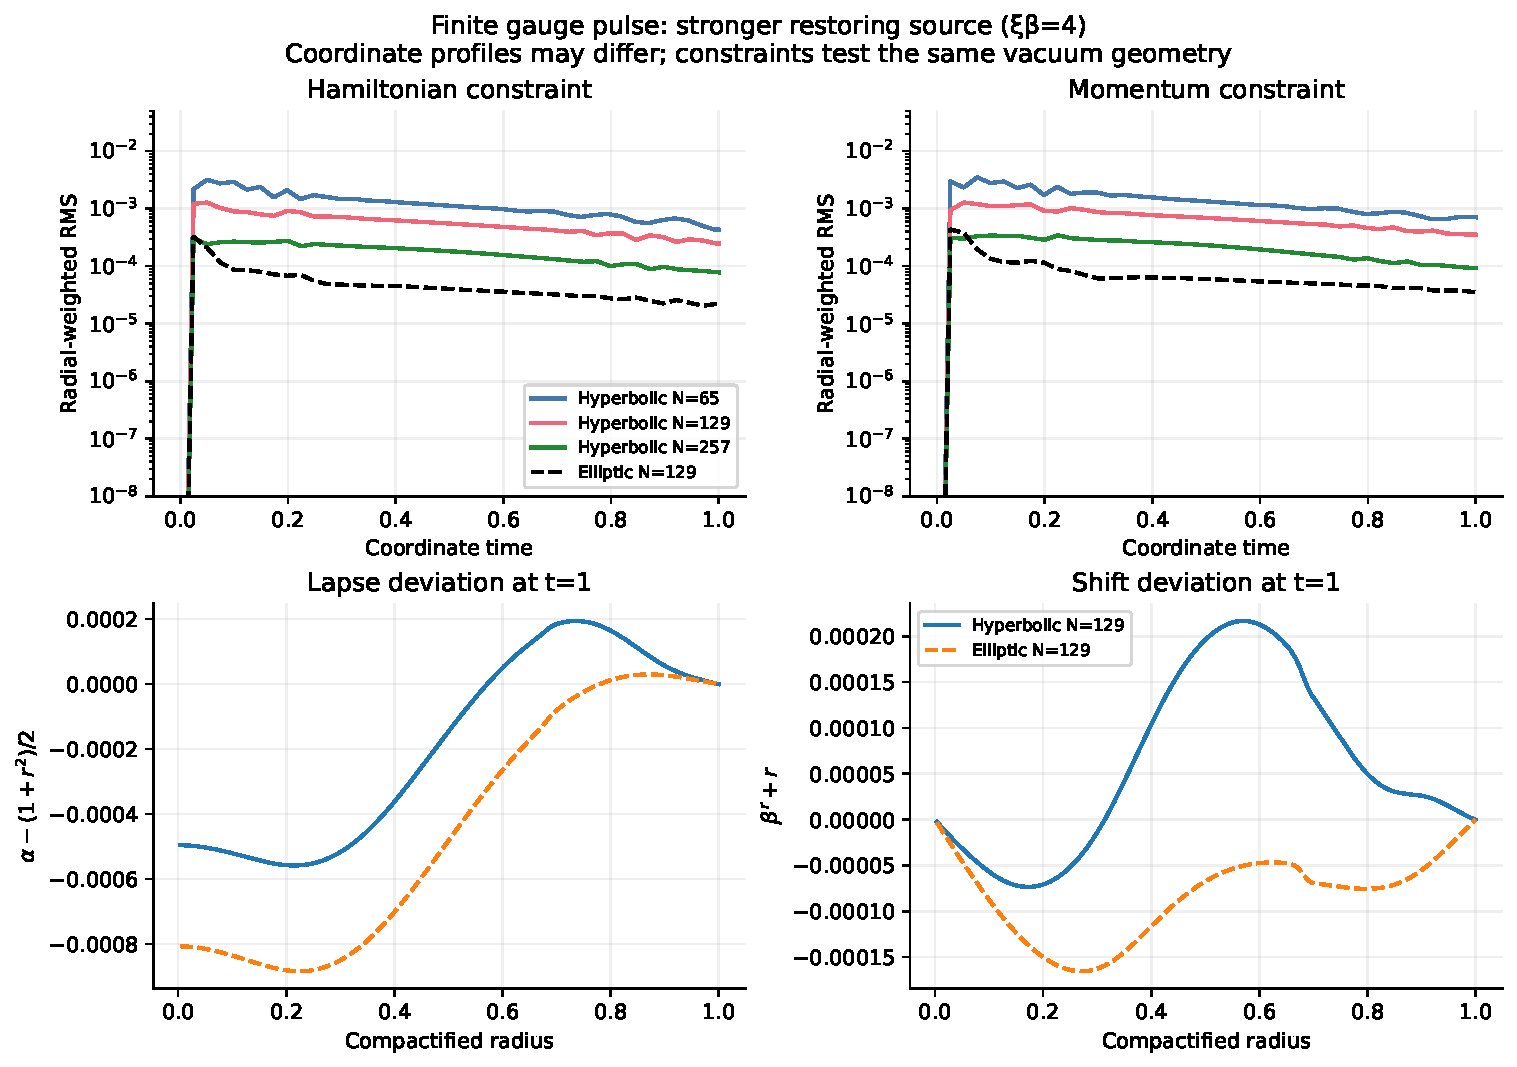
\includegraphics[width=\linewidth]{figures/pulse-comparison.pdf}
\caption{Finite pulse with $\xi_\beta=4$. Constraint errors decrease under refinement. The lower panels illustrate different coordinate responses, without interpreting their difference as physical error.}
\end{figure}
\FloatBarrier

\section{Failures, puncture treatment, and qualification decision}
Without restoring, the $N=65$ pulse violates the predeclared exploratory scri-numerator threshold $10^{-2}$ at $t=0.248062$. Varying the speed ratio, increasing auxiliary damping, or halving KO strength did not remove that failure. With $\xi_\beta=1$, $N=65$ and $257$ reach $t=1$, but $N=129$ fails at $t=0.249027$. This nonmonotonic behavior is preserved rather than called convergence. The stronger source succeeds in the regular-center refinement sequence above.

Linearized method-of-lines spectra at Minkowski, $N=33,65$, have negative spectral abscissae for the three tested restoring strengths. Thus these spectra do not explain the nonlinear pulse failures as an already demonstrated exponentially growing linear eigenmode. Nonnormal amplification, nonlinear boundary compatibility, and finite-resolution coupling remain possible mechanisms. Exact nullness is maintained even in every failed trajectory.

\begin{figure}[htbp]
\centering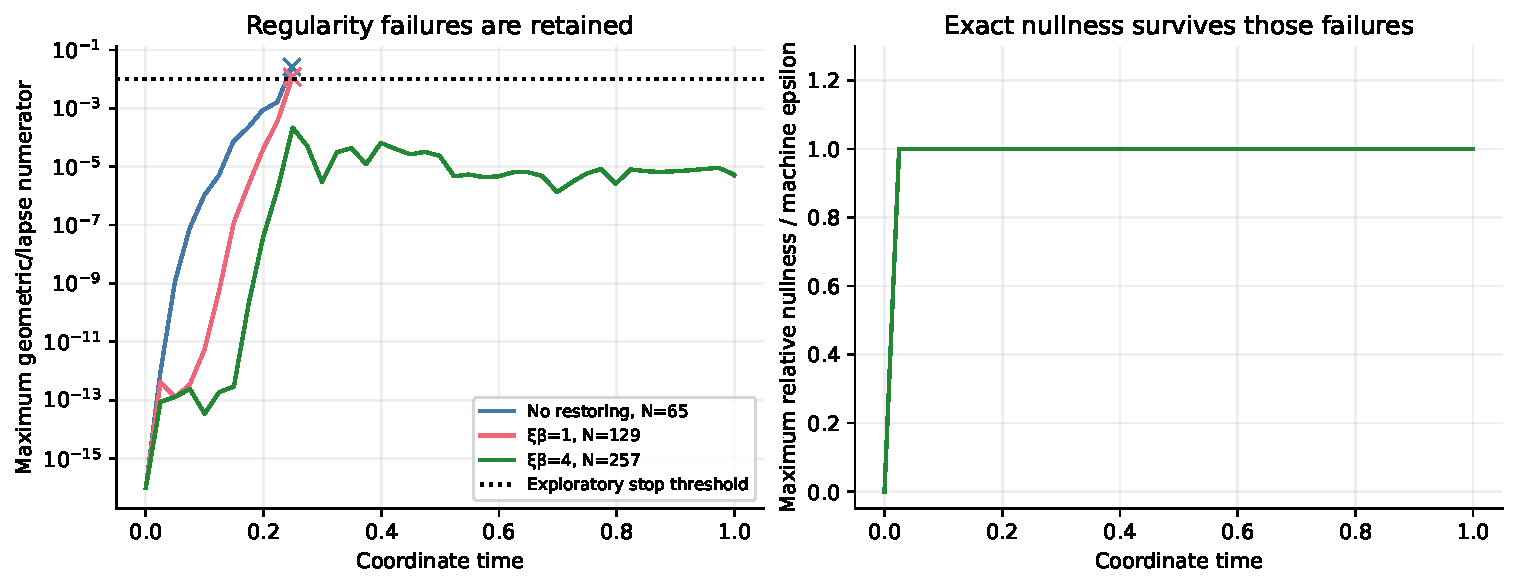
\includegraphics[width=\linewidth]{figures/boundary-failures.pdf}
\caption{Failed controls and a surviving regular-center candidate. Crosses mark actual stop states. The nullness diagnostic accumulates over all RK stages and accepted states; it does not imply cancellation of the other scri numerators.}
\end{figure}

The wormhole trials preserve $M=1/3$ and the baseline matched isotropic initial slice. They retain the radial map with stretch 16, positive-node stencils, reference-weighted positive variables, and physical lapse floor $10^{-10}$. All positive-radius nodes evolve; none are excised. The RK lapse variable is the total conformal lapse. Accepted increments use compensated accumulation. A separate total-value tensor adapter avoids subtracting small lapse, conformal factor, and physical trace from reference values. The initial shift is matched to the elliptic datum; subsequent stages use only the local driver.

The coefficient endpoint is rederived for $g=1+g_1r+\cdots$ and $\beta=b_1r+b_2r^2+\cdots$. In particular,
\begin{equation}
 \partial_t\Lambda_0=2b_1\Lambda_0-4b_1g_1+\frac{16}{3}b_2,\qquad
 \partial_t g_1=b_1g_1+\frac43b_2.
\end{equation}
The leading logarithmic $\chi$ and lapse rates remain $2b_1$ and $2b_1-6+2\xi(0)$. Independent tensor evaluations approaching $r=0$ converge to these coefficient limits. This checks the leading expansion, not a uniformly accurate puncture evolution.

Fresh trials use $\xi_\beta=4$ and $\Delta t\leq0.0125h$. At $N=129$ the scri guard stops the evolution at $t=0.19423828125$; $N=257$ reaches its short target $t=0.2$. The final relative errors with respect to analytic $M$ are $7.7463\times10^{-4}$ and $3.9726\times10^{-6}$, respectively. Maximum mass changes relative to each numerical initial horizon mass are $1.1975\times10^{-3}$ and $1.2846\times10^{-5}$. Two unequal-duration grids do not establish puncture convergence or wormhole-to-trumpet relaxation.

For exterior constraints, the mask uses the instantaneous apparent horizon and the RMS is normalized by the sum of exterior radial quadrature weights. The full interior diagnostics are retained separately. At the final saved states the interior maximum $|H|$ is $0.449$ and $0.00164$. The largest used-minus-original rate differences are in $\Lambda^r$ near $r=3.65\times10^{-8}$ and $1.60\times10^{-8}$, of order $4.64\times10^4$ and $2.01\times10^4$. These include the finite-difference advection and dissipation modifications, not an independent continuum residual. They prevent an accuracy claim near the puncture. The floor activates only inside $r\simeq6.29\times10^{-7}$.

The independently evaluated raw lapse-clock rates at the final endpoints are $0.0276$ and $-0.00438$, despite the imposed $\alpha_t=0$. These compatibility defects, together with the scri numerators, are a reason to revisit the boundary closure. They do not identify a unique cause of failure. The later bounded duration probes below reassess this short-test decision; no 3D run has been launched.

\begin{figure}[htbp]
\centering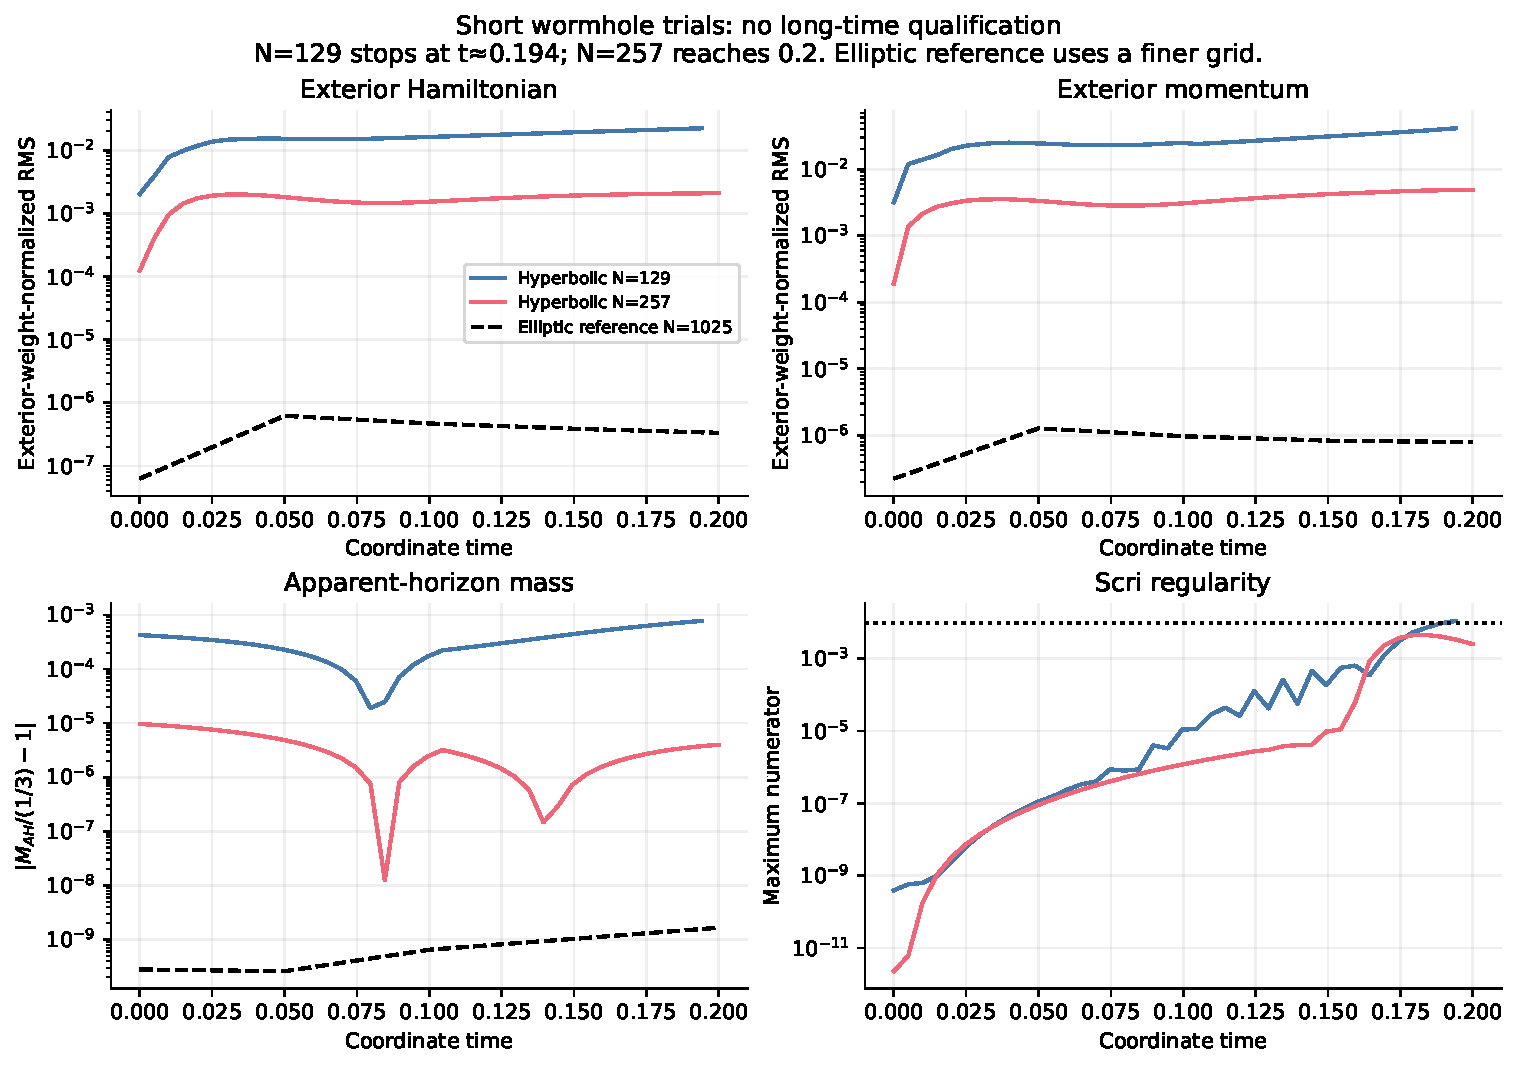
\includegraphics[width=\linewidth]{figures/puncture-comparison.pdf}
\caption{Short puncture tests. The dashed elliptic reference is $N=1025$, so this is not a matched-resolution superiority comparison. Mass errors include the initial discretization error; changes from the numerical initial mass are reported separately in the text.}
\end{figure}
\FloatBarrier


\section{Bounded extensions toward the persistent \texorpdfstring{$100M$}{100M} target}
The duration target is $t/M=100$, or coordinate $t=100/3$ for the retained $M=1/3$. The goal remains active. The predeclared criteria require three nested grids to reach that duration, decreasing exterior constraints and mass errors, positive-order field self-convergence, a separate timestep check, and continued positivity on every positive-radius node. A small horizon-mass error alone cannot certify a usable evolution.

At coordinate $t=1=3M$, grids $N=257,513,1025$ all complete with $\Delta t=0.05h$. Comparing $\Delta t=0.05h$ against $0.0125h$ at $N=257$ changes the final conformal lapse by at most $3.5\times10^{-13}$ and the horizon mass by $2.1\times10^{-14}$. This bounds the measured time sensitivity; two stepsizes do not establish a new temporal order.
\begin{center}
\begin{tabular}{rrrrr}
\toprule
$N$ & exterior $H$ RMS & exterior $M_r$ RMS & $|M_{\rm AH}/M-1|$ & peak scri numerator\\
\midrule
257 & $9.49\times10^{-3}$ & $1.86\times10^{-2}$ & $2.92\times10^{-5}$ & $4.90\times10^{-3}$\\
513 & $9.81\times10^{-4}$ & $9.12\times10^{-4}$ & $1.10\times10^{-6}$ & $2.99\times10^{-3}$\\
1025 & $4.33\times10^{-4}$ & $5.37\times10^{-5}$ & $5.81\times10^{-8}$ & $1.77\times10^{-3}$\\
\bottomrule
\end{tabular}
\end{center}
The full radial-weighted mixed-field self-differences are $1.7606\times10^{-2}$ and $1.3080\times10^{-2}$, giving only order $0.43$ at this time. The independently evolved connection dominates this mixed norm. These are short-time refinement results, not a satisfactory long-time convergence certificate. No puncture neighborhood is removed from the profile comparison.

Two fresh extensions target coordinate $t=3=9M$. The $N=257$ run stops at $t=2.825$ when its scri numerator exceeds $10^{-2}$. Its interior Hamiltonian maximum has already reached $3.19\times10^4$ near $r=0.0672$. The $N=513$ run fails earlier, at last accepted time $t=2.726953125$, because the next RK stage produces $g=-5.91\times10^{-6}$ near $r=0.09365$. A one-step postmortem replay reproduces that failure. The finer run's scri numerator remains below $0.0051$, so raising the scri guard would not cure this failure. The last scheduled diagnostics precede a between-sample stage failure; manifests and terminal arrays retain their separate exact times.

Both runs retain small horizon-mass drift: the largest sampled changes relative to their numerical initial masses are $2.77\times10^{-4}$ and $1.07\times10^{-5}$. Nevertheless, the loss of positive spatial metric makes the second run unusable. The failing region is far outside the lapse-floor radius, at most $7.32\times10^{-6}$. An outer-collar Jacobian diagnostic has negative spectral abscissae at the sampled times, but its artificial inner interface and exclusion of the bulk prevent a full-domain stability conclusion.

\begin{figure}[htbp]
\centering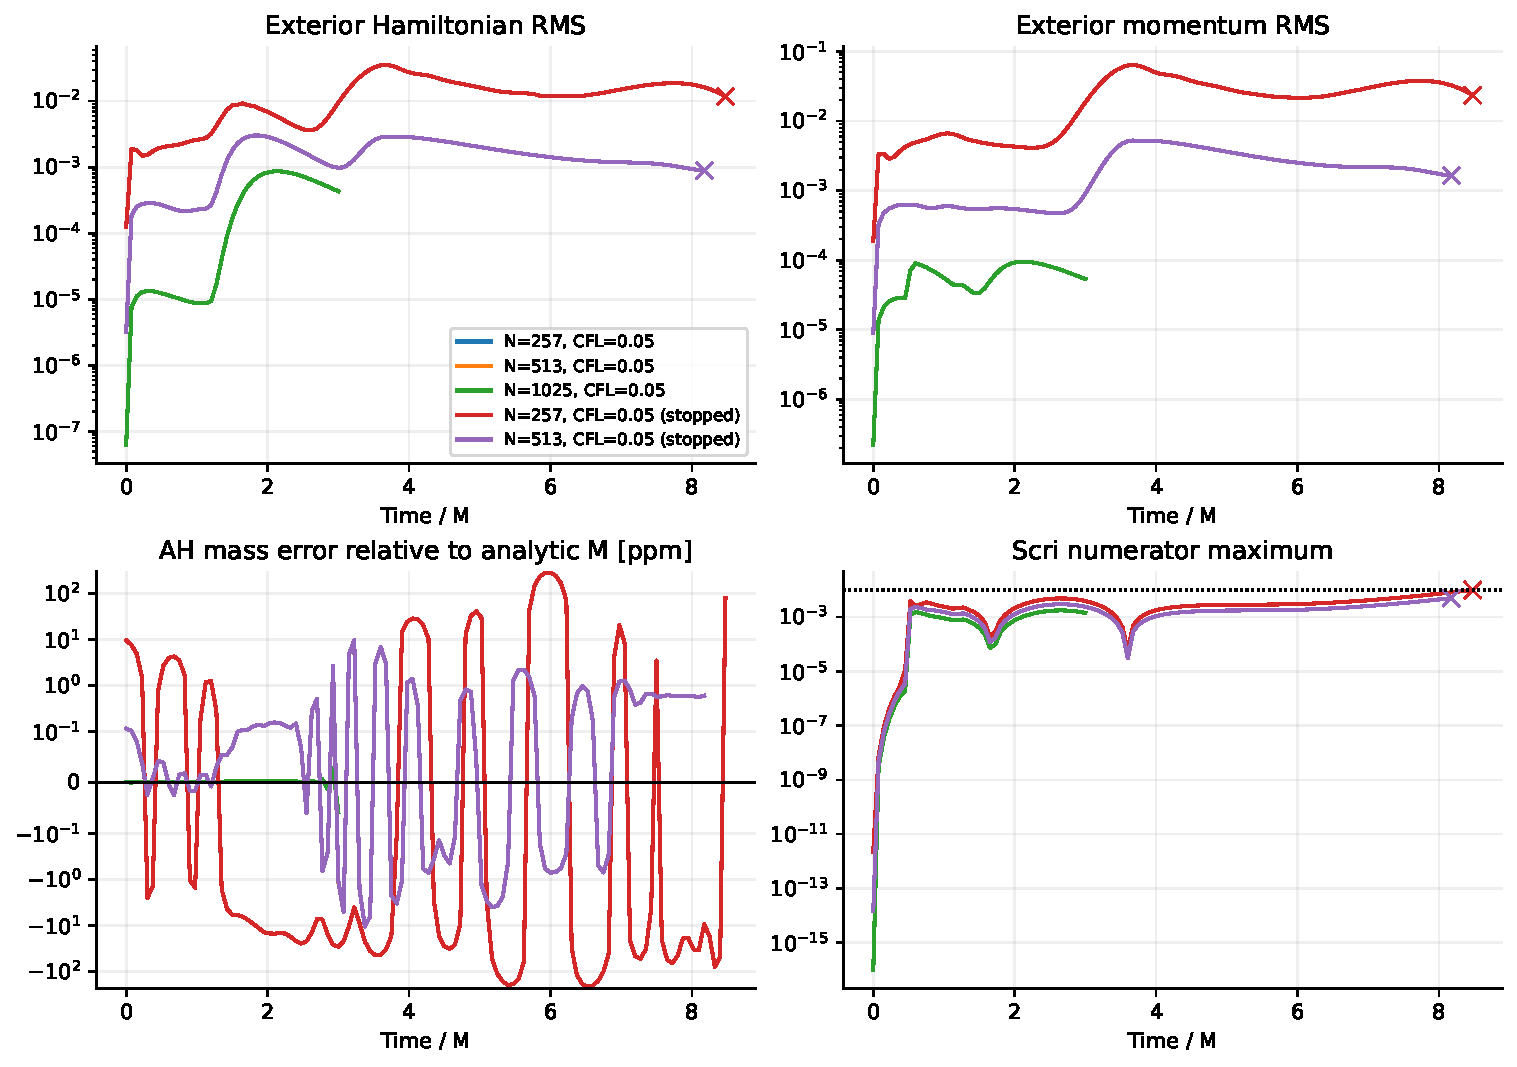
\includegraphics[width=\linewidth]{figures/duration-constraints.pdf}
\caption{Duration probes with the original hyperbolic driver. Curves terminate at their actual saved diagnostic times; crosses identify failed runs. The $N=1025$ trajectory is only a $3M$ probe. The horizon-exterior norms decrease with refinement, while interior metric breakdown still prevents continuation toward $100M$.}
\end{figure}
\begin{figure}[htbp]
\centering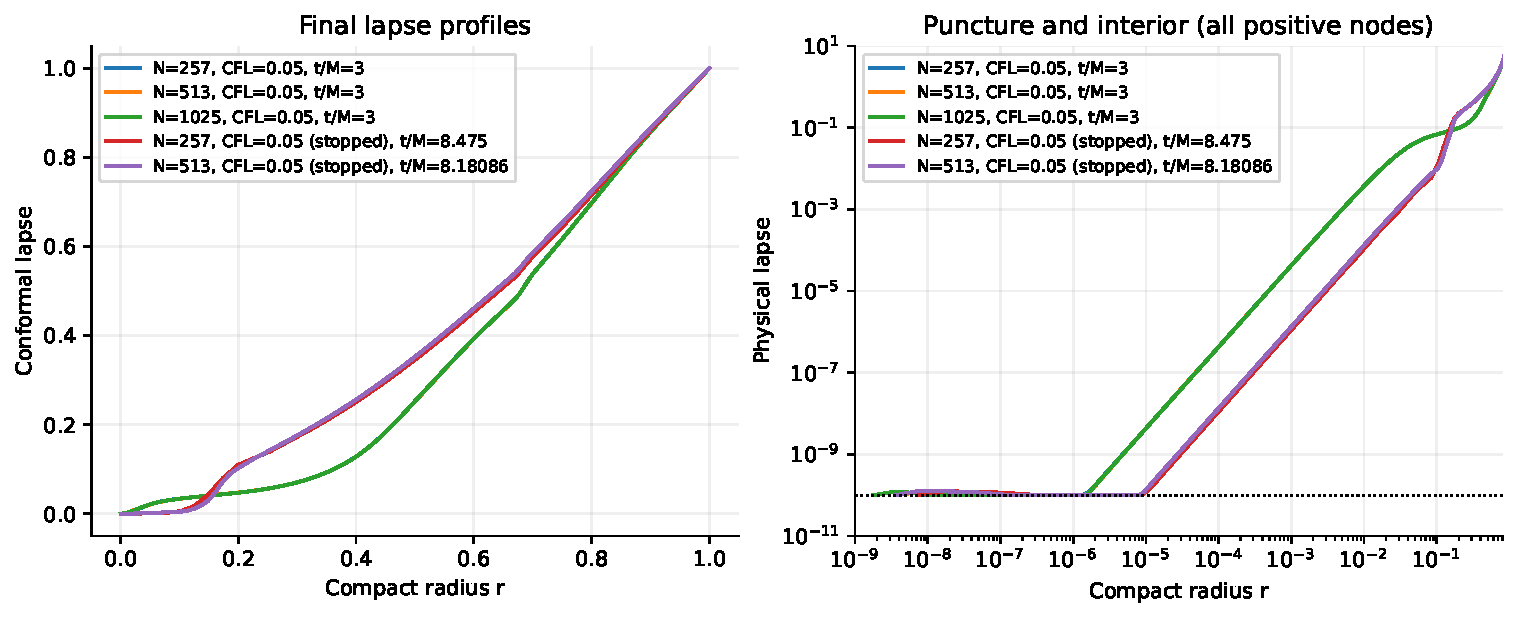
\includegraphics[width=\linewidth]{figures/duration-lapse.pdf}
\caption{Lapse snapshots at the indicated times, retaining the telegrapher coupling and physical floor $10^{-10}$. Different terminal times must not be interpreted as a convergence comparison. The floor region is several orders of magnitude closer to the puncture than the observed metric failure.}
\end{figure}
\FloatBarrier

A bounded candidate adds $b\Omega^2\sqrt\chi$ to $\mu$, with $b=0.1$. It leaves the scri coefficient and incoming-mode count unchanged and gives
\begin{equation}
 c_S^2=2c_L^2+\frac{4b\Omega^2\sqrt\chi}{3g}>2c_L^2
 \quad(\Omega>0,\ \chi,g>0).
\end{equation}
Before lapse flooring changes the leading AF scaling, the shift speed changes from $O(r^3)$ to $O(r)$. This is a gauge-transport hypothesis, not a cure established by the symbol. Three regular-center grids pass the same short gate, but the fresh $N=257$ puncture trial fails at $t=2.8078125$ when a stage metric becomes negative near $r=0.0672$. This candidate therefore does not resolve the duration failure and is not the default.

A mechanism tested next is the collapsed-region background forcing. For smooth AF data with $\beta=b_1r+O(r^2)$, the original driver gives, at continuum leading order,
\begin{equation}
 \dot b_1=b_1^2-1-2\xi_\beta(b_1+1).
\end{equation}
At $\xi_\beta=4$ this has a stable fixed point $b_1=-1$. Thus the driver actively restores the inward reference shift even in the collapsed-lapse region. The added $b\Omega^2\sqrt\chi D=O(r^2)$ does not change this leading forcing. This motivates the controlled source changes below; an increased survival time alone does not establish a unique cause of the original failure.

The implementation now writes atomic progress records and bounds diagnostic spacing by $\Delta t_{\rm report}\leq0.025$. A diagnostic-only optimization omits constraint and horizon calculations during intermediate RHS evaluations while retaining them at reports; the native rate arrays agree bit for bit with diagnostics enabled. Full failed-stage arrays are preserved for newly instrumented failures. The original failed runs and elliptic reference remain unchanged.


\subsection{Lapse-dependent shift sources and a metric-connection control}
The telegrapher lapse, its $\eta\chi$ attenuation, and the physical lapse floor remain unchanged in every control here. We replace only the shift background terms by
\begin{equation}
 \dt\beta=-r\sigma^2+\mu D-\xi_\beta\frac{\beta+r\sigma}{\Omega}.
\end{equation}
The global choice is $\sigma=\alpha/A$. Its complete restoring limit is $\xi_\beta[\beta'+(r\sigma)']$; the $\sigma'$ term must be included when eliminating the dependent $D$ trace. Algebraic nullness still holds at each stage, but the $N=257$ global-source trial fails its scri guard at coordinate $t=0.175$. We retain that failure.

The interior-only choice is $\sigma=1+w(\alpha/A-1)$, using the existing smooth window. It equals $\alpha/A$ near the puncture and exactly one for $r\geq0.8$. Hence the original source and boundary closure are unchanged throughout the outer collar. The change is algebraic in the evolved fields, so the interior principal matrix is unchanged. Before flooring alters the AF expansion, the leading slope equation becomes
\begin{equation}
 \dot b_1=b_1^2-2\xi_\beta b_1,
\end{equation}
whose stable fixed point is zero. Independent tests verify the leading AF rate and full scri limit, the unperturbed Minkowski equilibrium, and roundoff nullness for perturbed stage data.

Three regular-center pulse grids pass their short gate with decreasing constraint errors. Fresh puncture grids $N=257,513$ both reach $t=3=9M$. Their exterior Hamiltonian RMS values are $9.91\times10^{-3}$ and $4.02\times10^{-4}$; their absolute relative horizon-mass errors are $1.81\times10^{-3}$ and $7.42\times10^{-5}$. These two-grid improvements do not establish convergence of the modified gauge through $100M$.

Both trajectories continue from verified checkpoints through $t=5=15M$. The subsequent extensions fail at $t=5.3609375$ and $5.6947265625$, respectively. A stage metric becomes negative near $r=0.00332$ on the coarse grid and $r=0.01156$ on the finer grid. The fine trajectory's maximum sampled horizon-mass drift is only $2.03\times10^{-4}$, and its last sampled exterior Hamiltonian RMS is $1.51\times10^{-3}$. These exterior diagnostics do not make a state with invalid spatial geometry evolvable. Interior constraint magnitudes are diagnostic evidence; the stopping condition is loss of metric positivity, not an interior error budget.

A separate gauge control sources $D$ from the metric-derived connection $V$, while continuing to evolve $\Lambda^r$ independently in the unchanged Z4 system:
\begin{align}
 \dt D&=\dt V-\eta_DD,\qquad
 G=\dt g=-2\alpha A_{rr}+\frac{4g}{3}(\beta'-\beta/r),\\
 \dt V&=\frac{G'+\beta'g'}{g^2}
 +\left[-\frac{2g'}{g^3}+\frac{g^{-1/2}+2g^{-2}}{r}\right]G
 +\frac{2\beta}{r^2}(\sqrt g-g^{-1}).
\end{align}
This is a local hyperbolic gauge source, not an elliptic solve or a replacement of $\Lambda^r$ by $V$ in the Einstein equations. The last principal-symbol row becomes $(-2\alpha/g^2)\partial_rA_{rr}+[4/(3g)]\partial_r^2\beta$. Exact factorization yields the same scalar polynomial as Eq.~\eqref{eq:poly}, with complete normalized-scri eigenspaces for $\lambda=2$ and the same degeneracy at $\lambda=1$. The full puncture and 3D well-posedness limitations remain.

A complex-step chain-rule oracle checks the metric-connection rate to $2.1\times10^{-16}$, and the metric rate agrees with the native tensor kernel to $5.6\times10^{-17}$ in the tested states. The implementation evaluates this continuum rate with central derivatives and gives $D$ its own biased transport and KO terms. Unlike the evolved-$\Lambda$ control, it does not feed numerical dissipation of $\Lambda$ into $D$. It passes the regular-center gate and the $N=257$ puncture test through $9M$, but subsequently loses metric positivity at $t=5.487109375$ ($16.46M$). It is therefore not a duration repair.

\begin{figure}[htbp]
\centering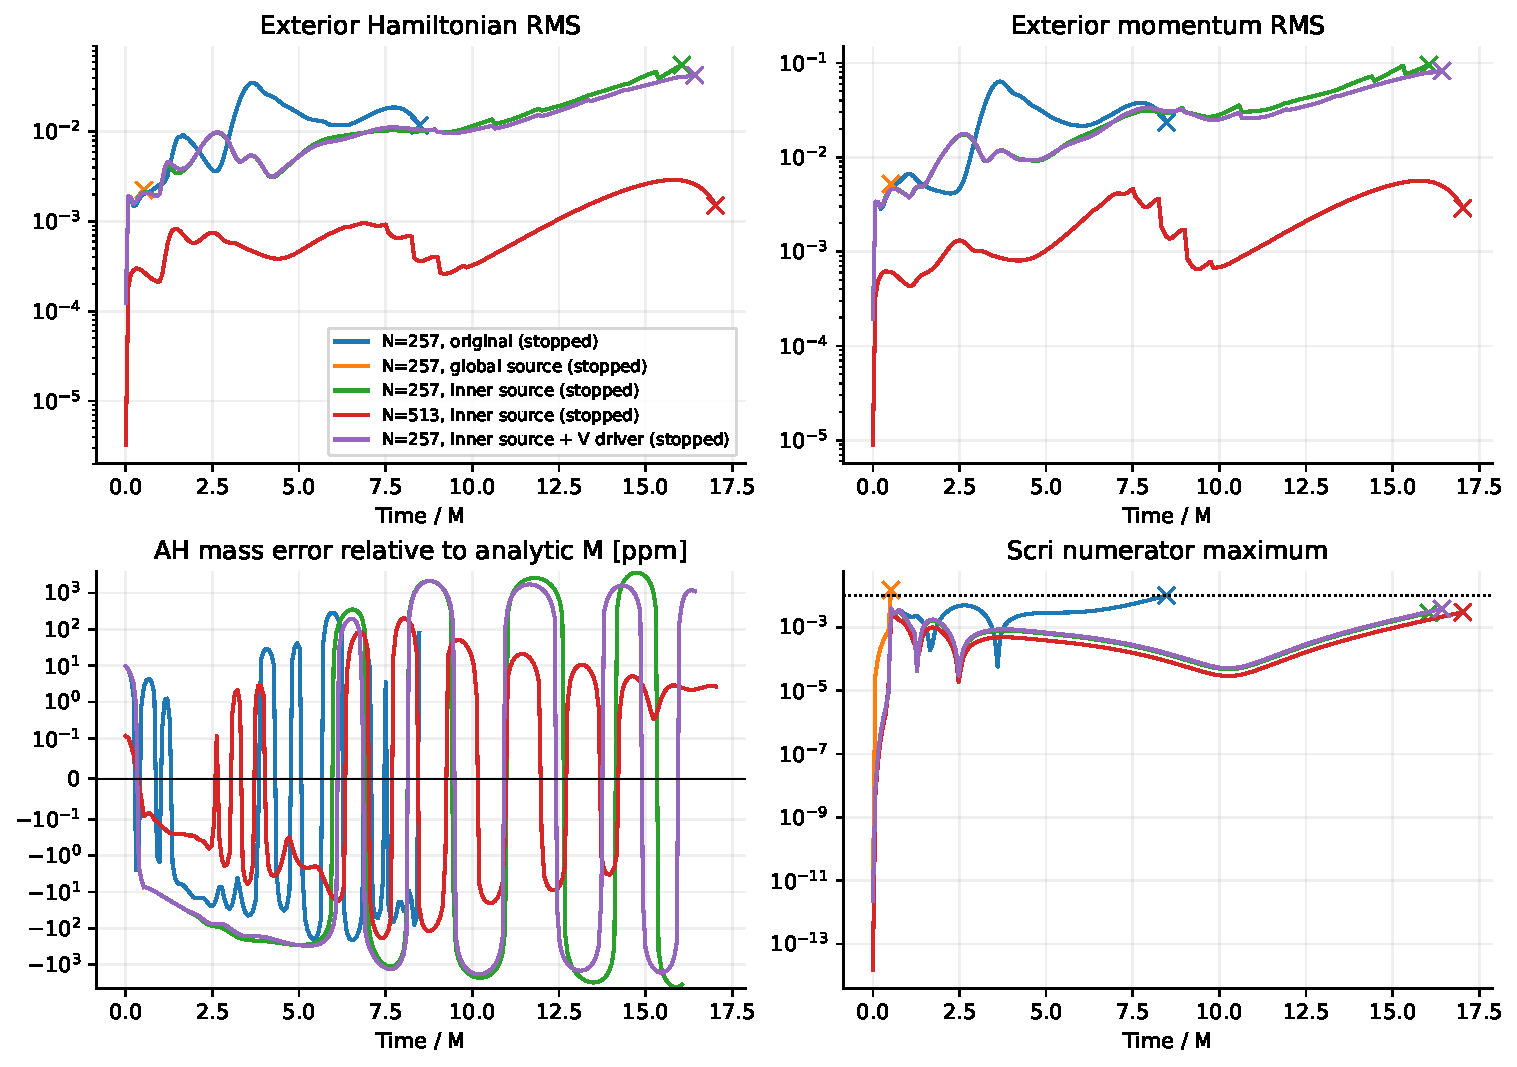
\includegraphics[width=\linewidth]{figures/source-constraints.pdf}
\caption{Failed source/driver controls, all retaining the telegrapher lapse. Each curve includes its verified continuation history. Crosses show the last saved diagnostics of a failed trajectory; exact last-accepted and failed-stage times are retained separately. The finer interior-source run has much smaller exterior errors but still fails before $18M$.}
\end{figure}
\begin{figure}[htbp]
\centering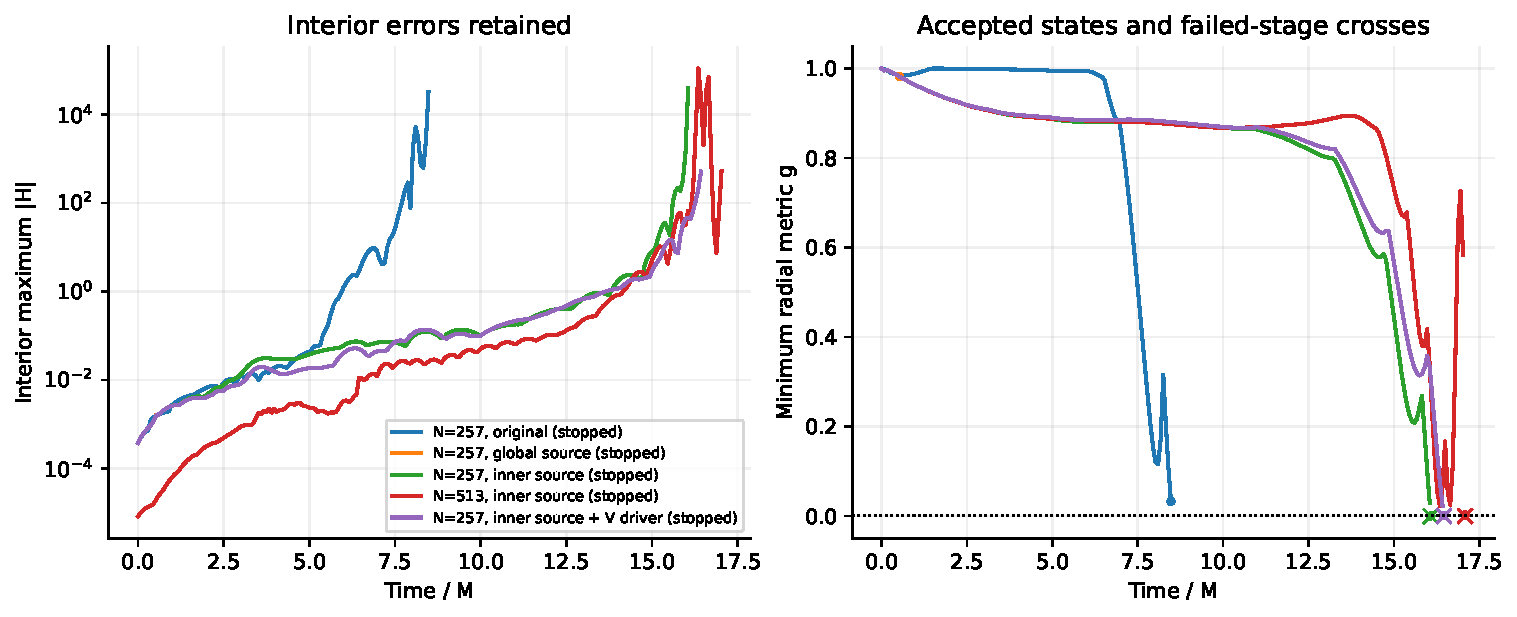
\includegraphics[width=\linewidth]{figures/source-interior.pdf}
\caption{Interior errors and metric positivity. Filled dots add the last accepted metric minimum; crosses in the metric panel use the actual failed-stage array when available. The global-source trial stops on its scri guard before developing the later interior failure. No interior nodes are removed from the evolution.}
\end{figure}
\begin{figure}[htbp]
\centering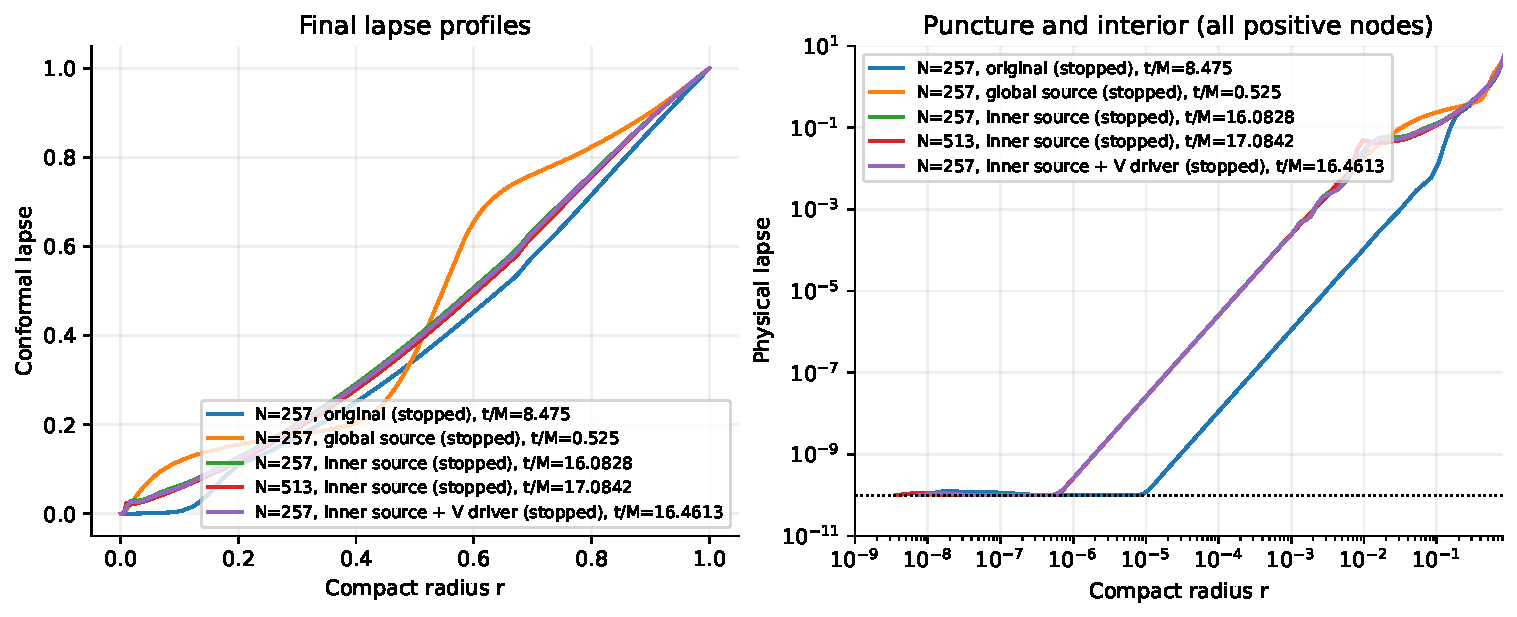
\includegraphics[width=\linewidth]{figures/source-lapse.pdf}
\caption{Final lapse snapshots for the same failed controls, at unequal times as labeled. The physical floor is retained. These profiles cannot serve as a common-time convergence test.}
\end{figure}
\FloatBarrier

The continuation harness accepts completed parents only, verifies source, library, checkpoint, and parent-record hashes, loads the frozen parent equations, and inherits the exact timestep and RK compensation. Two-generation split/uninterrupted tests agree bit for bit. A test initially exposed a one-ulp difference caused by recomputing $\Delta t=t_{\rm end}/N_t$; fresh runs now preserve the nominal $\mathrm{CFL}\,h$ bit pattern when the target is on that lattice. Corrupt histories, changed sources, failed parents, and unaligned continuation targets are rejected. These short restart tests establish implementation consistency, not long-time physical accuracy.

A possible later numerical control is to use $\log g$ and the mixed curvature $A_{rr}/g$ as evolution variables. That change would require a separate chain-rule/native-kernel audit, including loss of precision in the current deviation-based tensor adapter when $g$ becomes very small. No metric floor or logarithmic-metric evolution has been used. The requested next direction instead restores a moving-puncture-like shift in the bulk, as described below. The $100M$ objective remains unmet.


\subsection{An unsuppressed bulk Gamma driver}
The next candidate follows the fully advective two-variable Gamma-driver structure in Eqs.~(18) and (20) of \href{https://arxiv.org/html/gr-qc/0605030v2}{van Meter et al. (2006)}. Its shift coefficient does not vanish with the lapse or conformal factor. Let $C(r)$ be zero for $r\leq0.8$, one for $r\geq0.9$, and $x^8/[x^8+(1-x)^8]$ in between, where $x=(r-0.8)/0.1$. We use
\begin{align}
 \dt\beta&=\mu_\Gamma D-r-4C(r)\frac{\beta+r}{\Omega},\\
 \dt D&=\dt\Lambda^r-D,\qquad
 \mu_\Gamma=(1-C)\mu_{\rm bulk}+C\mu_{\rm separated}.
\end{align}
Here $\mu_{\rm separated}$ is the earlier coefficient with $\lambda=2$. Thus the bulk has a constant-strength advective Gamma driver and no reference-restoring force. The prescribed $-r$ source remains necessary to preserve the chosen hyperboloidal Minkowski equilibrium with $D=0$; this is a disclosed difference from the asymptotically flat gauge. No measured Einstein-equation residual is subtracted. The outer collar recovers the previous driver and its complete scri limit exactly. The algebraic normal shift and dependent auxiliary trace are imposed at every stage as before; no additional scri datum is supplied.

The coefficient is configurable. The conventional $\mu_{\rm bulk}=3/4$ is not used for the first evolution: with the retained telegrapher lapse at the Minkowski center, $c_L^2=1=4\mu_{\rm bulk}/3$. Exact rational eigenspace calculations give algebraic multiplicity two but geometric multiplicity one for each of the speeds $\pm1$. Setting $\mu_{\rm bulk}=1$ separates those speeds and gives complete scalar eigenspaces at that state. The general polynomial remains Eq.~\eqref{eq:poly}, with the new $\mu_\Gamma$. At normalized scri there are still one incoming, six outgoing and three tangent scalar modes. At the exactly collapsed corner $\alpha=\chi=0$, the zero eigenvalue has algebraic multiplicity eight and geometric multiplicity seven even with this unsuppressed driver. No uniform collapsed-lapse or full 3D strong-hyperbolicity claim follows.

For $N=257$, the original stretch-16 map would give a mapped gauge speed of $5.66\times10^5$ and a Courant number of $2.83\times10^4$ at $\Delta t/h=0.05$. The new puncture controls therefore explicitly set the map strength to zero, retain the C7 outer grid collar, and use $\Delta t/h=0.025$. The first positive radius is then $1/256$, rather than $7.49\times10^{-9}$. This is a different grid family; improved duration on it cannot isolate the gauge change from the mesh change.

The implementation audits confirm an exact bulk shift-rate identity, unchanged native Einstein and telegrapher-lapse rates at identical states, independent evolution of $\Lambda^r$, and stage nullness below $2.3\times10^{-16}$. The regular-center Minkowski residual is $1.47\times10^{-13}$. Three finite-pulse grids complete through $t=1$, with mixed-field self-differences $2.374\times10^{-3}$ and $6.252\times10^{-4}$, corresponding to an approximate order of $1.925$. An independent fixed-grid pulse test at $t=0.15$ uses $\Delta t=0.0015,0.00075,0.000375$ and gives temporal order $4.004$. This is a short regular-center result, not long puncture temporal convergence.

The first puncture implementation retained positive-node extrapolation for shift derivatives. Its coarse $N=257$ run reached $t=0.2$, but $N=513$ lost metric positivity at $t=0.149462890625$, at the third positive node. Halving the timestep gives a failure at $t=0.1494873046875$, again at the third positive node. The near-identical failure time and reversal under spatial refinement reject that implementation as a stable candidate. A separate reduced radial-vector wave test isolates the leading gauge equation,
\begin{equation}
 \partial_t^2\beta+\partial_t\beta=\frac{4\mu_{\rm bulk}}3
 \left(\beta''+\frac{2\beta'}r-\frac{2\beta}{r^2}\right),
\end{equation}
about the collapsed, zero-shift leading state, with the same KO8 coefficient and four fixed outer nodes. This isolates the singular inner spatial closure; background advection and the complete coupled geometry are omitted. Positive-node extrapolation gives maximum growth rates $26.16$ and $52.68$ on $N=65,129$. An odd radial-vector extension gives maximum real eigenvalues approximately $-0.5$ on both grids. This reduced spectral test identifies a closure instability; it is not a stability proof for the complete Einstein system.

The resulting control uses odd extension only for shift and auxiliary derivatives. At the fixed spherical puncture, $\beta(0)=0$ implies $D(0)=0$ through the unsuppressed shift equation; the auxiliary value is dependent, not an extra independent gauge datum. The AF geometry, lapse, curvature, and independent connection retain their positive-node stencils and are not assigned regular-center parity. All positive-radius nodes remain evolved. With that closure, all three puncture grids $N=257,513,1025$ reach $t=0.2=0.6M$. The horizon-exterior Hamiltonian RMS values are $1.623\times10^{-3}$, $2.767\times10^{-4}$, and $1.299\times10^{-5}$; the interior maxima are $7.508\times10^{-4}$, $5.665\times10^{-5}$, and $2.706\times10^{-6}$. Full-domain mixed-profile self-differences give an approximate order of $3.69$ at this short common time. The lapse floor does not activate in these resolved-grid tests. This does not assess the very small radii sampled by the earlier stretch-16 grid, nor establish convergence through $100M$.


Verified continuations reach $t=3=9M$ on both $N=257,513$. At this common time, exterior Hamiltonian RMS decreases from $6.822\times10^{-3}$ to $5.865\times10^{-4}$ and momentum RMS from $1.362\times10^{-2}$ to $1.154\times10^{-3}$. The fine-grid final relative horizon-mass error is $-8.66\times10^{-10}$, with maximum sampled drift $4.21\times10^{-8}$. No third grid has yet reached this duration, so these improvements are not a long-time convergence certificate.

The coarse trajectory continues to $t=8=24M$, beyond the earlier source-control failures. Its final relative horizon-mass error is $-2.98\times10^{-6}$, maximum sampled mass drift $6.42\times10^{-6}$, and exterior Hamiltonian RMS $5.40\times10^{-3}$. However, the minimum metric has fallen to $0.459$ at the first positive node, and the interior Hamiltonian maximum is $1.12\times10^2$ near $r=0.0156$, inside the horizon at $r\simeq0.154$. These are unresolved signs of interior deterioration. They are retained as diagnostics rather than used as an interior constraint budget. The physical geometry remains valid at the terminal checkpoint, and no floor activation occurred.

All these runs maintain relative nullness within $2.23\times10^{-16}$. The sampled quantity $g(c_S^2-c_L^2)$ remains positive, with minima about $0.260$ and $0.267$ in the coarse and fine continuations. This excludes a sampled lapse/shift speed crossing along those trajectories; it does not prove uniform eigenvector bounds. The next priority is longer matched refinement with this bulk driver, including whether the late inner degradation moves or decreases with resolution. The $100M$ stability and convergence goal remains open.

\begin{figure}[htbp]
\centering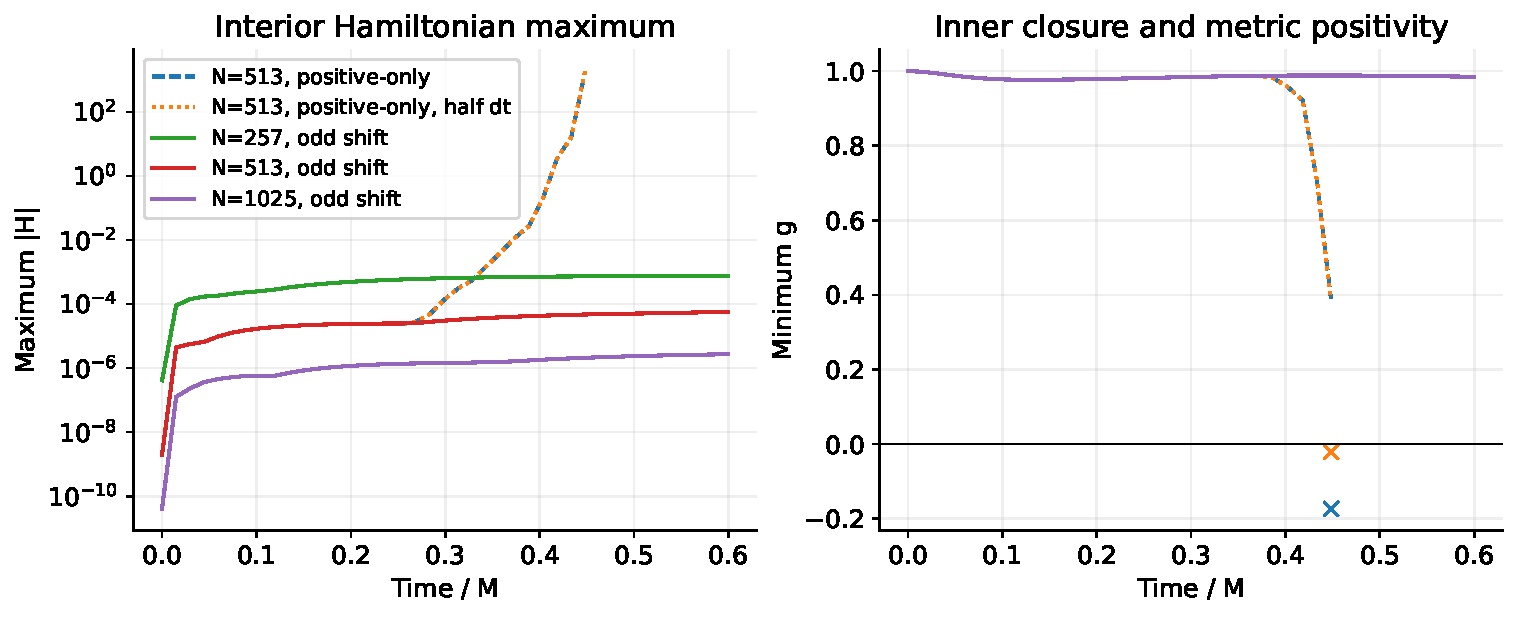
\includegraphics[width=\linewidth]{figures/gamma-inner-closure.pdf}
\caption{The fast Gamma wave exposes an unstable positive-only inner gauge stencil. Halving the timestep leaves the early failure nearly unchanged. Odd extension of the shift variables removes this short-time failure on three grids; puncture geometry retains its positive-node stencils. Crosses show actual failed-stage metric minima.}
\end{figure}
\begin{figure}[htbp]
\centering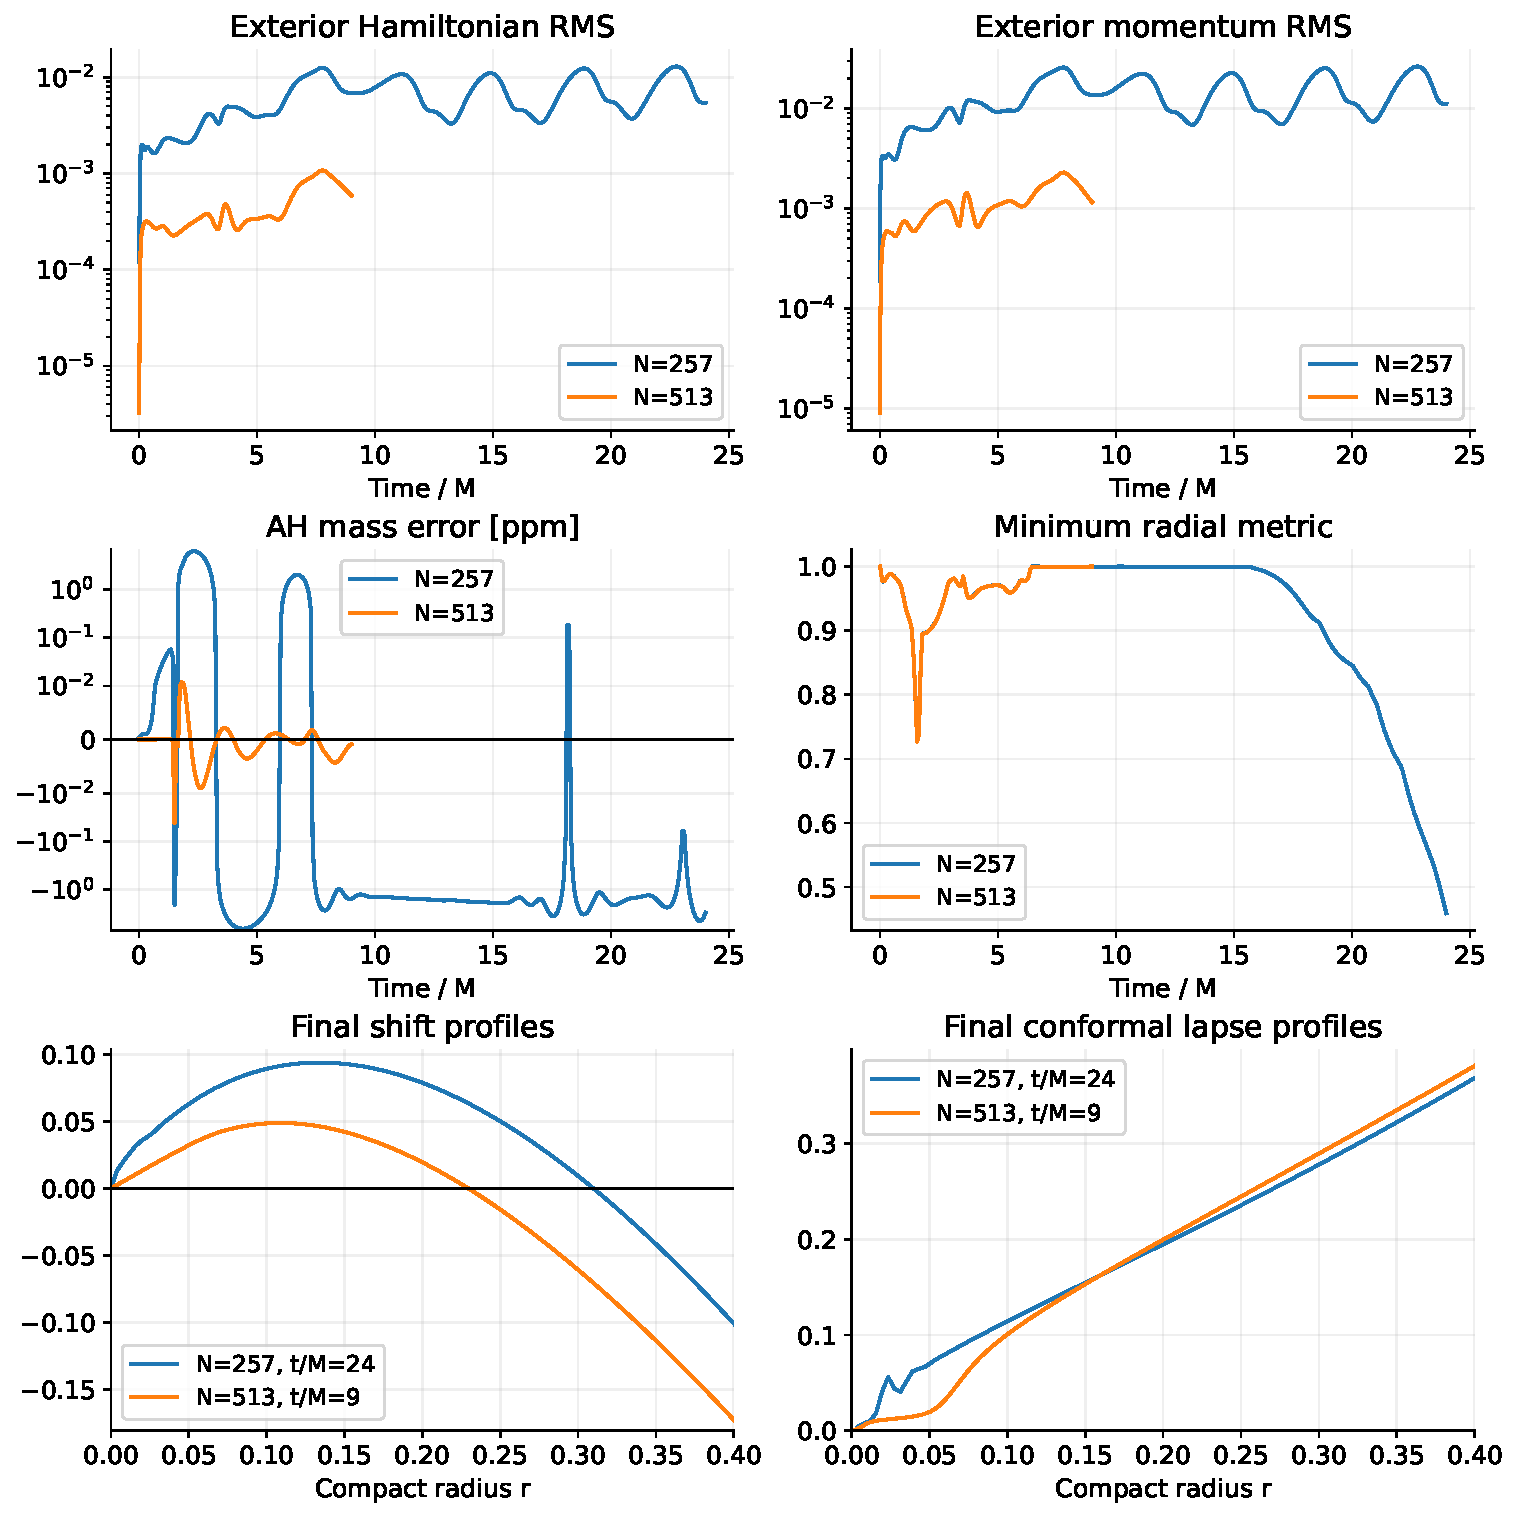
\includegraphics[width=0.94\linewidth]{figures/gamma-progress.pdf}
\caption{Unsuppressed bulk Gamma-driver continuations with the revised inner gauge closure. Exterior constraints are normalized over apparent-horizon-exterior radial weights. The coarse run survives to $24M$, but its metric minimum deteriorates after about $15M$. Final inner shift and lapse snapshots are at unequal times, as labeled, and are not a convergence comparison. The outward interior shift is now allowed to develop.}
\end{figure}
\FloatBarrier

\section{Implementation route and reproducibility}
A genuine 3D implementation should evolve Cartesian shift and auxiliary vectors in the interior and transform them consistently to shell frames. The spherical code evolves the full radial component, not a globally slaved $\beta/r$ profile. Spherical symmetry necessarily fixes the central location; it is not a test of puncture motion. Constant and linear Cartesian shift modes must be included in the 3D driver tests. The reference source and restoring term can influence translations, so their effect on puncture tracking must be measured rather than assumed benign.

At a cubed-sphere outer face, compute $s_i$ from the live regular metric and the analytic $\Omega_i$. Eliminate the normal shift component after every stage, ghost fill, prolongation, restriction, and synchronization. Derive the corresponding auxiliary compatibility trace in that frame. Specify tangential coordinates only after counting the vector-sector characteristics. A normal nullness identity alone supplies no tangential gauge condition.

Before deployment, derive a direction-independent 3D version of the telegrapher coupling and speed coefficient, and audit all scalar, vector, and tensor eigenvectors for arbitrary positive metrics. The present radial $g$-dependent speed separation is not yet such a 3D prescription. AMR needs stage-consistent characteristic interface treatment, stable dissipation across refinement boundaries, and nullness reconstruction after interpolation; a boundary component should not be interpolated as an independent scalar. Shell interfaces additionally require tensor/connection transformation and reference-connection checks. Moving punctures require positive-variable interpolation, measured floor effects, and resolution studies of the near-puncture constraint and gauge fields.

The implementation is under \path{tst/hyperbolic_shift_1d/}; frozen inputs are under \path{inputs/hyperbolic_shift_1d/}. Each run records its command, source hashes, library hash, input values, stop reason, histories, and profiles. Failed runs retain their actual outcomes. Portable exports are under \path{docs/hyperbolic-shift-1d/evidence/}; complete per-run source snapshots and libraries remain in the ignored local output tree. The original elliptic implementation is unchanged except for an additive native adapter with unchanged legacy entry points; all 24 independent $g=1$/tensor comparison cases still pass.

\begin{center}
\begin{tabular}{p{0.25\linewidth}p{0.65\linewidth}}
\toprule
Evidence category & Established scope\\
\midrule
Analytic identities & Nullness elimination, evolving-normal rate, scalar principal polynomial, selected exact eigenspaces, leading AF limits.\\
Algebraic numerics & Every tested stage/state satisfies spherical nullness within one machine epsilon; general 3D boundary identities have separate randomized tests.\\
Convergence evidence & Short regular-center refinement; three-grid new-gauge puncture evidence through $0.6M$ and earlier-gauge evidence through $3M$; no $100M$ convergence certificate.\\
Unresolved & Complete boundary well-posedness, uniform collapsed-lapse hyperbolicity, accurate puncture evolution, long-time robustness, and all 3D/AMR qualification.\\
\bottomrule
\end{tabular}
\end{center}
The practical outcome is a reproducible experimental alternative with a working exact-nullness mechanism. It is not a replacement for the successful elliptic configuration.
\end{document}
